\chapter[Nonradiative Decay Mechanisms in 2'-hydroxychalcones]{Nonradiative Decay Mechanisms\\ in 2'-hydroxychalcones}
\label{chapter:NRdecay}
\section{Introduction}\label{section: NRdecay_intro}
Computational methods have the potential to explain the intriguing luminescence properties of the \acf{HC} derivatives introduced in Section \ref{section: lom HC}. \textbf{HC} derivatives \textbf{1}-\textbf{5} of Figure \ref{figure: HC_experimental} have strikingly different emission characteristics in the solid state, for which we wish to disentangle the intra- and intermolecular contributions. This chapter addresses the intramolecular interactions present in the five systems. The effect of the substituents on the four level \ac{ESIPT} photocycle are analysed through a combination of static and nonadiabatic dynamics simulations, investigating the relaxation mechanisms and the competition between different deactivation channels. These simulations show that a strong electron donating group (EDG) in the \textit{para} position alters the topology of the potential energy surface (PES), destabilising the \Estar{} state, thereby assisting and accelerating proton transfer. Our results provide detailed understanding into the fundamental relaxation mechanisms of \ac{HC}s and the role of the substituents, which is the initial step in unravelling the effect of aggregation on the emission properties.

This work presented in this chapter was published in reference\citenum{Dommett2017}. The structure of this chapter follows that of the published article. The computational methods used shall be described, followed by analysis of the vertical excitations, minima on the excited state, and the feasible relaxation channels. Finally the results of nonadiabatic dynamics rationalise those obtained in static calculations. The relevant Supporting Information of ref.\citenum{Dommett2017} is incorporated into the chapter and designated appendices.

\section{Computational Methods}\label{section: NRdecay_methods}
The ground state geometries of all the compounds were optimised in vacuum using resolution of identity \acf{MP2} with the def2-SV(P) and def2-TZVP basis sets.\cite{Haase1993,Schafer1992,Weigend2005} Vertical excitation energies were calculated in vacuum using coupled cluster to approximated second order (CC2) and \acf{ADC2} methods under the resolution of identity approximation with the def2-TZVP basis set.\cite{Christiansen1995,Hattig2000,Hattig2002,Kohn2003,Hattig2005} Core electrons were frozen for all \ac{MP2}, \ac{ADC2} and CC2 calculations. The performance of the ADC(2) and CC2 methods is compared, whilst the effect of the basis set is considered for ADC(2). 

Geometry optimisation in the first excited state was carried out in vacuum for \textbf{1}-\textbf{5} with ADC(2) and CC2 methods using the same basis sets as the ground state optimisation. These calculations were performed with Turbomole v7.0.\cite{Turbomole} The level of theory considered to discuss the features of the surfaces is CC2/def2-TZVP, unless otherwise specified.

The CIOpt software package of Levine, Coe, and Martinez was used to determine the location of the \acf{MECI} structures.\cite{Levine2008} The MECI structures were obtained for \textbf{1}-\textbf{5} at the CC2/def2-TZVP, ADC(2)/def2-TZVP, and ADC(2)/def2-SV(P) levels of theory. In the case of \textbf{1}, \ac{CASSCF} calculations were performed with MOLPRO program.\cite{Molpro} The \sone/\szero{} conical intersections were optimised with state-averaged CASSCF (SA-CASSCF). The active space considered 12 electrons in 11 orbitals (CASSCF(12,11)) including 2 states in the average with the 6-31G(d) basis set. The CASSCF(14,13) active space was also considered. These spaces are shown in Appendix A. The \acp{PES} were explored through \ac{LIIC} pathways with ADC(2)/def2-TZVP level of theory. In the case of \textbf{1}, the intermediate \ac{LIIC} geometries were relaxed with the $\theta_{tor}$ angle fixed at the CC2/def2-TZVP level of theory. The geometries along the intersection seam were located using CIOpt. 

The absorption spectra of \textbf{1}-\textbf{5} were simulated using the nuclear ensemble method. 500 nuclear configurations were generated based on a Wigner distribution of the harmonic frequencies calculated at MP2/def2-SV(P) level of theory.\cite{Crespo-Otero2012} Five excited states at ADC(2)/def2-SV(P) level of theory were calculated for each individual geometry. For \textbf{1} and \textbf{5}, \acf{TSH} non-adiabatic dynamics simulations were performed using NEWTON-X interfaced with Turbomole, at ADC(2)/def2-SV(P) level of theory.\cite{Barbatti2014} The initial conditions for the dynamics were generated from the absorption spectra considering an energy window of $\pm$ \si{0.15} {eV} in the absorption spectra, simulating laser excitation.\cite{Barbatti2007} The geometries contributing to these energy windows were used as initial for the trajectory propagation along with their velocities and momenta. \szero{}, \sone{}, and \stwo{} states were included in the dynamics. 

For compound \textbf{1}, an energy window at absorption maximum of 3.35 $\pm$ 0.15 eV was selected for the nonadiabatic dynamics. 50 trajectories were statistically distributed between \sone{} (30) and \stwo{} (20), according to their oscillator strengths. The same protocol was used for compound \textbf{5}, with 50 trajectories (\sone: 30 and \stwo: 20) from an energy window of 3.39 $\pm$ 0.15 eV. The maximum simulation time was 500 fs, with a time step of 0.5 fs and the quantum equations were integrated with 0.025 fs using interpolated quantities between classical steps. Non-adiabatic effects were included using the fewest-switches surface hopping algorithm with decoherence corrections (0.1 Hartree). Non-adiabatic couplings between \stwo{} and \sone{} were estimated approximately using an approximated wave-function and the numerical method.\cite{Ryabinkin2015} The trajectories were terminated when the energy gap between \sone{} and \szero{} was less than 0.1 eV.

\section{Results}\label{section: NRdecay_Results}

\subsection{Vertical Excitations}\label{section: NRdecay_VE}
\begin{table}[t]
    \centering
    \begin{tabular}{cccccccccccc}
    \hline
     & \multicolumn{3}{c}{ADC(2)/def2-SV(P)} & & \multicolumn{3}{c}{ADC(2)/def2-TZVP} & & \multicolumn{3}{c}{CC2/def2-TZVP}\\
    \hline
     State & $\Delta$E & \textit{f} & Character & & $\Delta$E & \textit{f} & Character & & $\Delta$E & \textit{f} & Character\\
    \hline
    & \multicolumn{11}{c}{Compound \textbf{1}}\\
     \hline
      \sone   & 3.53 & 0.604 & \pipistar & & 3.36 & 0.869 & \pipistar & & 3.43 & 1.135 & \pipistar\\ 
      \stwo   & 3.58 & 0.391 & \npistar & & 3.44 & 0.090 & \npistar  & & 3.67 & 0.009 & \npistar \\
      \sthree & 3.97 & 0.013 & \pipistar  & & 3.77 & 0.008 & \pipistar & & 3.84 & 0.003 & \pipistar\\ 
      \hline
     & \multicolumn{11}{c}{Compound \textbf{2}}\\
     \hline
     \sone   & 3.53 & 0.483 & \pipistar  & & 3.38 & 0.806 & \pipistar & & 3.43 & 1.167 & \pipistar  \\ 
     \stwo   & 3.59 & 0.551 & \npistar  & & 3.46 & 0.196 & \npistar &  & 3.68 & 0.023 & \npistar \\
     \sthree & 3.96 & 0.010 & \pipistar  & & 3.77 & 0.007 & \pipistar &  & 3.85 & 0.005 & \pipistar \\ 
     \hline
     & \multicolumn{11}{c}{Compound \textbf{3}}\\
     \hline
     \sone   & 3.59 & 1.022 & \pipistar & & 3.40 & 1.063 & \pipistar  &  & 3.47 & 1.286 & \pipistar \\
     \stwo   & 3.64 & 0.075 & \npistar  & & 3.51 & 0.013 & \npistar   &  & 3.75 & 0.002 & \npistar \\
     \sthree & 4.06 & 0.046 & \pipistar & & 3.86 & 0.038 & \pipistar  &  & 3.96 & 0.034 & \pipistar \\ 
      \hline
     & \multicolumn{11}{c}{Compound \textbf{4}}\\
     \hline
     \sone   & 3.53 & 0.404 & \pipistar & & 3.36 & 0.857 & \pipistar &  & 3.42 & 1.105 & \pipistar  \\
     \stwo   & 3.57 & 0.589 & \npistar  & & 3.42 & 0.096 & \npistar  &  & 3.65 & 0.005 & \npistar  \\
     \sthree & 3.86 & 0.002 & \pipistar & & 3.65 & 0.008 & \pipistar &  & 3.72 & 0.028 & \pipistar \\ 
     \hline
     & \multicolumn{11}{c}{Compound \textbf{5}}\\
     \hline
     \sone   & 3.42 & 0.647 &\pipistar & & 3.20 & 0.522 & \pipistar  & & 3.26  & 0.633 & \pipistar  \\
     \stwo   & 3.52 & 0.012 &\npistar  & & 3.39 & 0.066 & \npistar & & 3.54 & 0.390 &  \pipistar\\
     \sthree & 3.67 & 0.337 &\pipistar & & 3.50 & 0.358 & \pipistar & & 3.66& 0.094 &  \npistar \\ 
     \hline
    \end{tabular}
    \caption[Vertical excitation energies of \textbf{HC1}-\textbf{5}]{Vertical excitation energies, oscillator strengths, and orbital character for compounds \textbf{1}-\textbf{5} at various levels of theory. The corresponding ground state was calculated with the MP2 method with the corresponding basis set. All energies are in eV.}
    \label{table: HC_VEs}
\end{table}

The vertical excitation energies for the first three excited states were calculated for structures \textbf{1}-\textbf{5} and are summarised in  Table \ref{table: HC_VEs}. Using CC2/def2-TZVP as reference, it is evident that the behaviour of \textbf{5} is somewhat different to \textbf{1}-\textbf{4}. In \textbf{1}-\textbf{4}, there is negligible substituent effect, with a bright \pipistar{} state predicted for \sone{}, where the energy varies by less than 0.05 eV across the four structures. \stwo{} is a dark \npistar{} state involving the carbonyl nonbonding pair, whilst \sthree{} is also a dark \pipistar{} excitation. In compound \textbf{5}, the first two excited states are \pipistar{} with a red shift of 0.17 eV compared to \textbf{1}, with the oscillator strength of \stwo{} increased at the expense of \sone{}, with the \npistar{} state shifted to \sthree{}. 

The electron density difference maps between \sone{} and \szero{}, Figure \ref{figure: HC_Vac_Densities},  reveal the origin of differing excitation pattern in \textbf{5}. For \textbf{1}-\textbf{4}, the excitation to \sone{} involves density transfer from the unsaturated bridge of the system (connecting the phenol and dimethylaniline rings) to the carbonyl \pistar{} orbital. For \textbf{5}, electron density is transferred not from the bridge but from the phenol ring, due to the electron-rich conjugation of the methoxy group. Considerable electron density is transferred from the hydroxyl oxygen, increasing the acidity of the proton. The \stwo{} state in \textbf{5} has the same character as \sone{} in \textbf{1}-\textbf{4}. Thus the strong electron donor in \textbf{5} perturbs the electron density with respect to the other four compounds, changing the character of the bright state with a greater electron depletion at the hydroxyl oxygen. This shall be shown to be important in the following sections as we analyse the relaxation in the excited state.
\begin{figure}[t]
\centering
  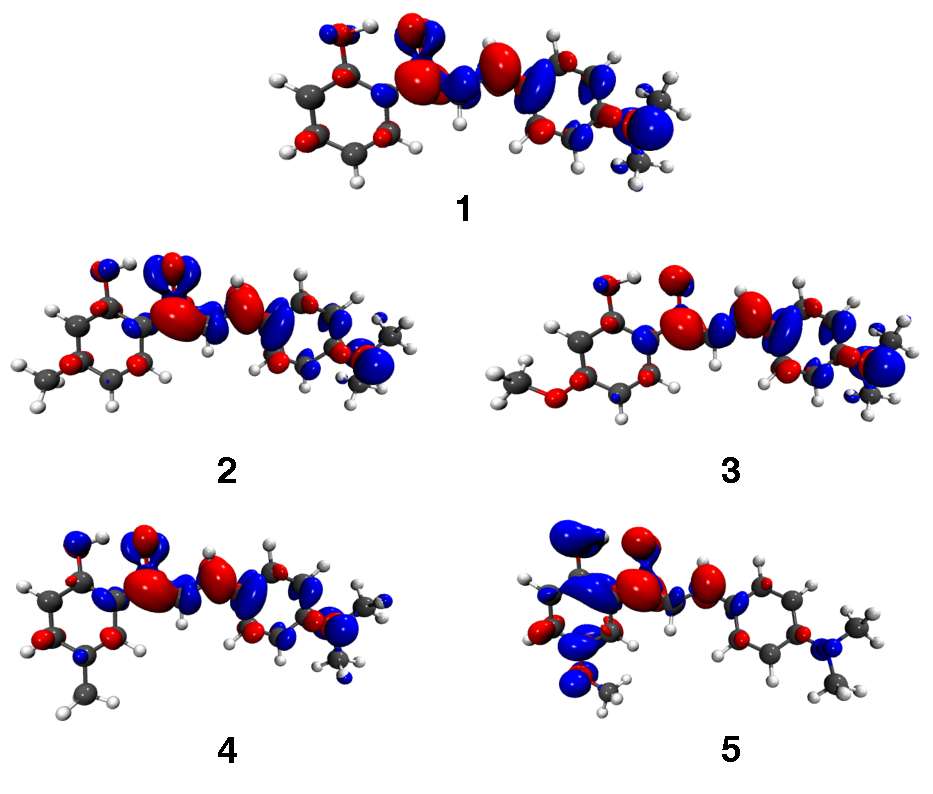
\includegraphics[width=0.8\linewidth]{3nonradiativedecay/HC_Vac_Densities.pdf}
  \caption[Electron density difference maps]{Electron density difference maps (\sone{}-\szero{}) for \textbf{1}-\textbf{5}, showing electron density loss in the ground state (blue) and gain in the excited state (red), calculated at CC2/def2-TZVP level of theory.}
  \label{figure: HC_Vac_Densities}
\end{figure}

Comparing the performance of ADC(2) and CC2 methods, when the same basis set is used (def2-TZVP), ADC(2) vertical excitation energies are about 0.1 eV deviated to the red with respect to the CC2 values. In the case of ADC(2), the def2-SV(P) basis set shifts the energies to the blue in about 0.1 eV. With this basis set there is mixing of the \sone{} and \stwo{} states, where \stwo{} borrows intensity from \sone{} due to  \pipistar{} and \npistar{} mixing, which is present in CC2 but to a lesser degree. The simulation of the spectra, Figure \ref{figure: HC_spectra_ADC}, using a Wigner-distributed sample of nuclear configurations at the ADC(2)/def2-SV(P) level of theory shows a red shift of 0.1-0.2 eV due to vibrational broadening. Similar shifts are expected for all levels of theory.
\begin{figure}[t]
\centering
  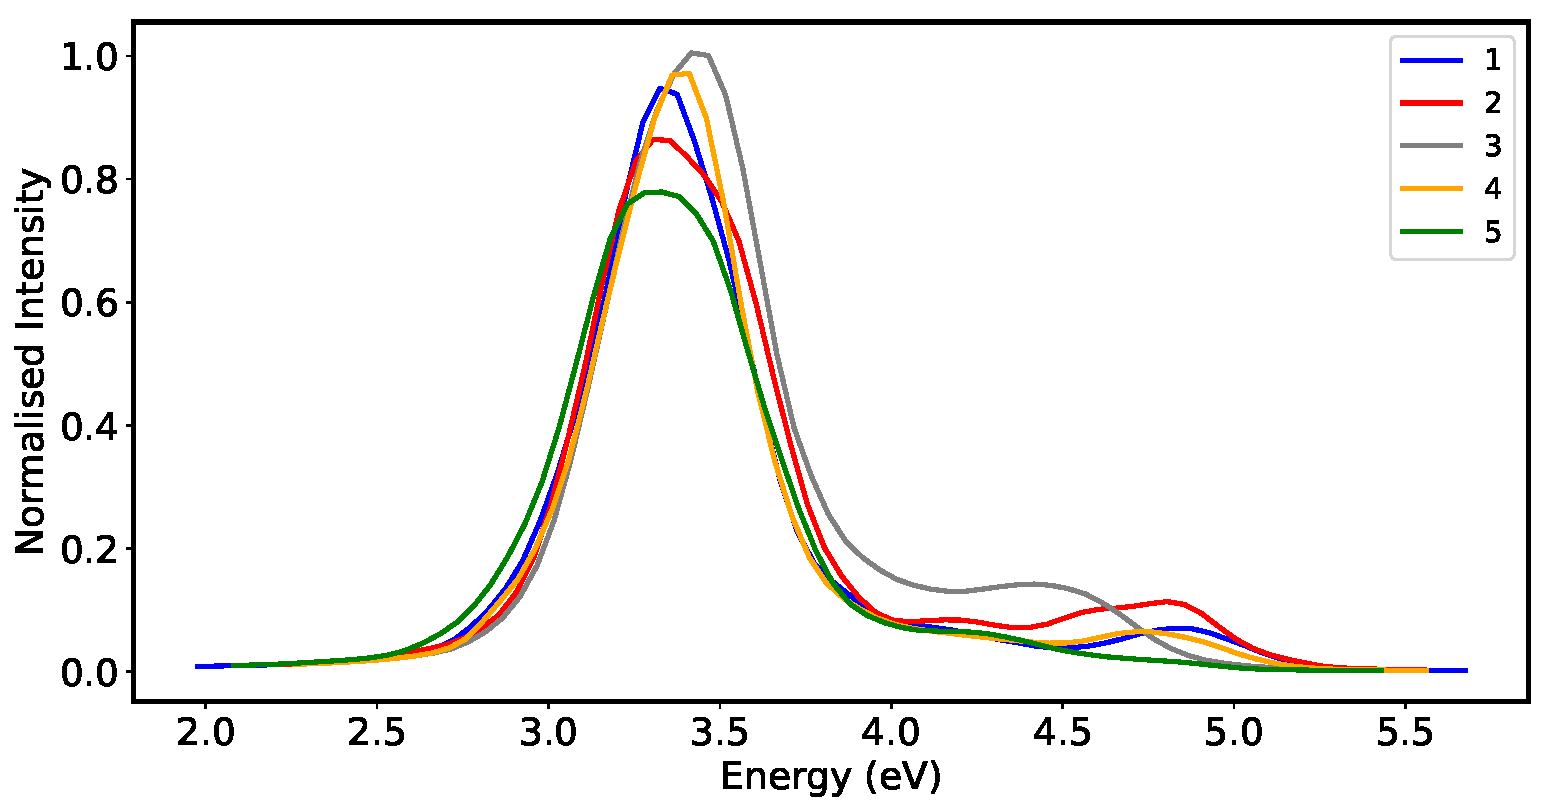
\includegraphics[width=0.8\linewidth]{3nonradiativedecay/HC_Spectra_ADC2.pdf}
  \caption[Simulated absorption spectra of \textbf{HC1}-\textbf{5}]{Simulated absorption spectra of \textbf{HC} \textbf{1}-\textbf{5} at ADC(2)/def2-SV(P) level of theory.}
  \label{figure: HC_spectra_ADC}
\end{figure}


\subsection{Excited State Minima}\label{section: NRdecay_Minima}
Minima in the first excited state for all compounds were optimised using ADC(2) and CC2 methods. The respective energy levels are depicted in Figure \ref{figure: HC_Energy_Levels}. An \ac{EDG} in \textit{meta} (\textbf{2} and \textbf{3}) has a negligible effect on the energies of \Estar. However, if the substituent is in \textit{para} (compounds \textbf{4} and \textbf{5}), no stable \Estar{} minimum can be located. For \textbf{1}-\textbf{3}, relaxation to a local minimum in \Estar{} is \textit{via} intramolecular rotation. To describe this mode, the torsional rotation angle $\theta_{tor}$ is defined in Figure \ref{figure: H_CC2_LIIC_Scan}.

Two \Estar{} minima can be found depending on the direction of rotation and in the case of \textbf{1}, both minima are energetically equivalent. For \textbf{1}-\textbf{3}, the energy difference between these minima is very small ($<$ 0.01 eV) and the two minima (forward or backwards rotation) can be considered degenerate. Torsion through 180\textdegree{} results in cis-trans isomerisation, with the trans isomer about 1 eV less stable than cis in \sone (at ADC(2), Figure \ref{figure: HC_1_Energylevels_ADC2}). Consequently, full cis-trans isomerisation is unlikely. 

At the \Estar{} minimum  $\theta_{tor}$ = 44\textdegree{} for \textbf{1}, resulting in  a stabilisation of approximately 0.54 eV with respect to the FC state. Compounds \textbf{2} and \textbf{3} pass through similar minima, with $\theta_{tor}$ = 46\textdegree{} and 54\textdegree{} respectively. Potential energy curves and our non-adiabatic dynamic simulations show that ESIPT from this geometry is improbable. Therefore when occupied the \Estar{} minimum acts as a sink for the wavepacket to prevent \ac{ESIPT}. The emission energies from the \Estar{} state for \textbf{1}, \textbf{2} and \textbf{3} are 1.63, 1.59, and 1.46 eV respectively, but with negligible oscillator strength.

In the \Kstar{} state, where the proton has migrated, the system relaxes \textit{via} intramolecular rotation about $\theta_{tor}$. Two minima with very similar energies can be also located depending on the direction of rotation. The $\theta_{tor}$ value ranges between 40\textdegree{} and 60\textdegree{}. These minima are about 1 eV below the excitation energy corresponding to the FC geometry, and are more stable than \Estar{} minima. As such a bias towards the ESIPT mechanism can be expected. An \ac{EDG} in \textit{para} (\textbf{4} and \textbf{5}) stabilises the \Kstar{} \sone{} state with respect to \textbf{1}, but the relative stabilisation with respect to the \sone{} energy for the FC geometry is quite similar for all the derivatives (about 1 eV). The emission from \Kstar{} is in the range of 0.7-1.0 eV for all molecules, but has negligible oscillator strength. \sone{} energies (for \Kstar{} and \Estar) with ADC(2) method are in good agreement the obtained with CC2 (within the 0.1-0.2 eV range). At the same time, ADC(2) destabilises the K ground state with respect the CC2 method. This behaviour has consequences for the optimisation of MECI and the description of the \sone/\szero{} crossing seam using the ADC(2) method, which are discussed in the next section.

\subsection{Relaxation Channels}\label{section: NRdecay_Channels}
\begin{figure}
\centering
  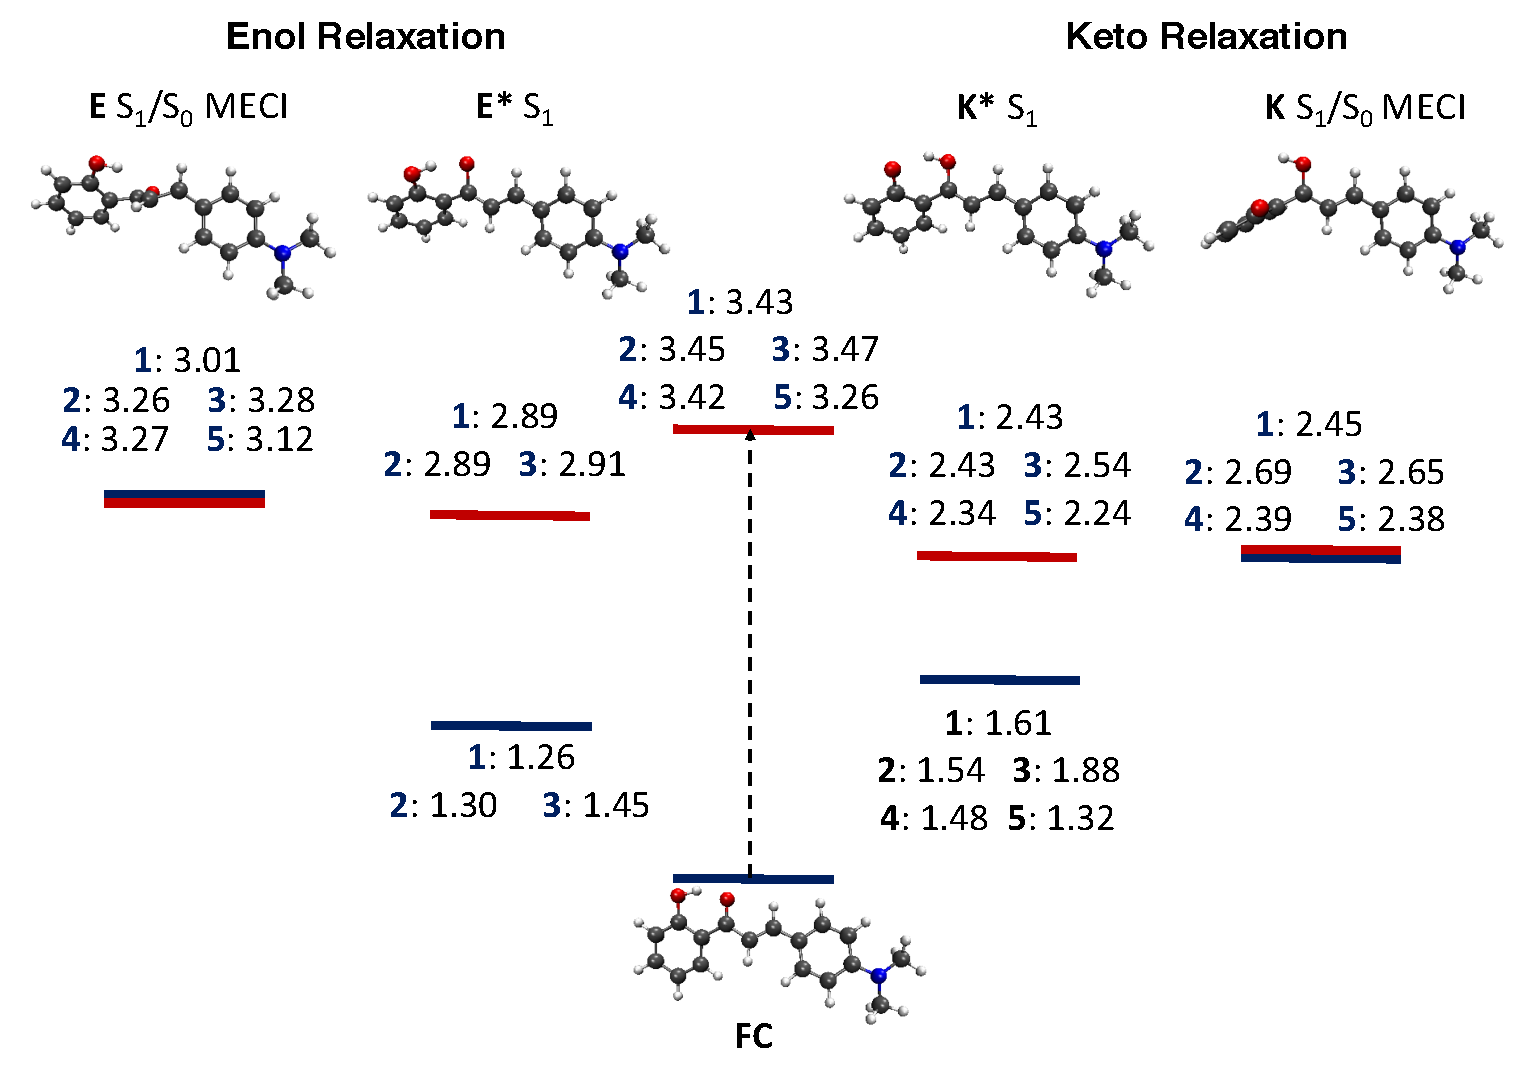
\includegraphics[width=0.9\linewidth]{3nonradiativedecay/HC_Energy_Levels.pdf}
  \caption[\textbf{HC} energy levels]{Relative energies (in eV) for all derivatives calculated at CC2/def2-TZVP level of theory. In all cases, the energy of the ground state was taken as reference.}
  \label{figure: HC_Energy_Levels}
\end{figure}
From the Franck-Condon state, the wavepacket can relax through the enol channel to the \Estar{} minimum, or the ESIPT channel to the \Kstar{} minimum. These two competing channels are depicted in Figure \ref{figure: HC_Energy_Levels}. In each channel, the \ac{MECI} was located to determine the feasibility of nonradiative decay \textit{via} a nonadiabatic crossing. For \textbf{1}, the \ac{MECI} geometries were optimised with CC2 methods using the def2-SV(P) and def2-TZVP basis sets. For comparison, the conical intersections were also located with CASSCF(12,11)/6-31G(d) and CASSCF(14,13) levels of theory. The geometry of the \Kstar{} \sone/\szero{} \ac{MECI} obtained with the CC2 method is in very good agreement with that obtained with CASSCF, $\theta_{tor}$=88\textdegree{} (89\textdegree{} with CASSCF method). The RMSD deviation between the two geometries is just 0.08 \AA. The geometries obtained with both basis sets are very similar. 

For \textbf{1}, the MECI lies at only 0.02 eV above the \Kstar{} minimum, whilst the substituents slightly increase the energy of the MECI (0.1-0.2 eV) in \textbf{2}-\textbf{5}. Nevertheless, the MECIs remain accessible during the relaxation. To determine if any barriers exist between the \Kstar{} minimum and the MECI, we optimise the intermediate states of a linear interpolated pathways, fixing $\theta_{tor}$, at CC2/def2-TZVP level of theory for \textbf{1}. This is shown in Figure \ref{figure: H_CC2_LIIC_Scan}. At the \Kstar{} minimum, $\theta_{tor}$ = 50\textdegree, and further 30\textdegree{} rotation takes the molecule to the intersection seam. In this region of the potential energy surface, the \sone{} energy does not change significantly with $\theta_{tor}$, which can be associated with an extended crossing seam as previously described by Robb \textit{et al}. in an analogous ESIPT system.\cite{Paterson2005}

\begin{figure}[t]
\centering
  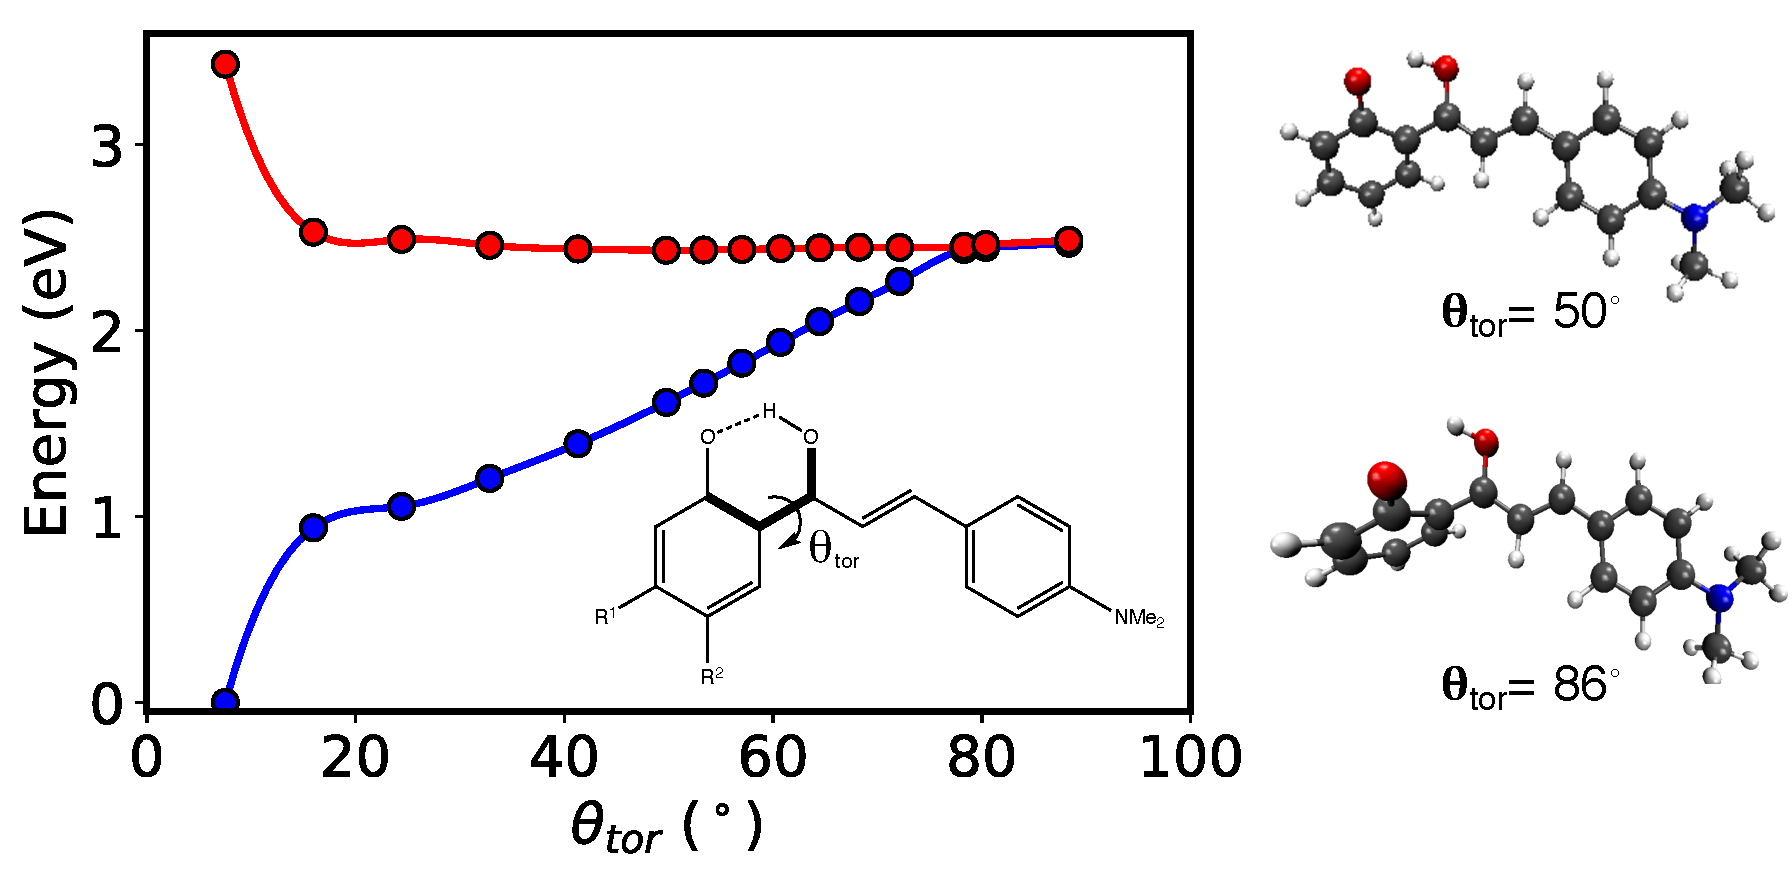
\includegraphics[width=0.9\linewidth]{3nonradiativedecay/H_CC2_LIIC_Scan.pdf}
  \caption[Potential energy surface along the relaxation mode $\theta_{tor}$]{Relaxed linear interpolation pathway between the FC state and the MECI. LIIC located six geometries between the FC state  \Kstar{} minimum, followed by LIIC to locate 10 geometries between the \Kstar{} minimum and MECI. All geometries were relaxed at CC2/def2-TZVP level of theory with $\theta_{tor}$ fixed.}
  \label{figure: H_CC2_LIIC_Scan}
\end{figure}

The frustration of intramolecular rotation in the solid state has been hypothesised to prevent access to a conical intersection, resulting in \ac{AIE}. We observe similar results when the dihedral angle is fixed during \Kstar{} optimisation. The linear interpolation potential energy curves show that there is a stable \Kstar{} region for \textbf{1} prior to the conical intersection, where emission could take place in the NIR region if the rotation is strongly hindered. The driving force behind the rotation is potentially the stabilisation of the dipole moment, which increases from 7.73 (\szero{}) to 13.32 D (\Estar) upon excitation. This is reduced to 3.99 D in the twisted conformation.

The static calculations suggest that the dominant relaxation process involves a proton transfer step followed by rotation about $\theta_{tor}$. ESPIT is facilitated by the \Kstar{} minimum, which is more stable than \Estar. Experimentally, \textbf{4} and \textbf{5} do not show fluorescence either in solution or solid state. In the case of the solid state, the lack of fluorescence has been associated with the crystal packing, however these calculations suggest that the character of the substituent might also play a role. This shall be further investigated in the next chapter.

The ADC(2) geometries for the \Kstar{} \sone/\szero{} MECI of all studied compounds show a $\theta_{tor}$ angle significantly deviated from CC2 and CASSCF values, with the crossing seam reached at a much smaller angle . The ADC(2) MECI structures are very similar to the \Kstar{} minima (deviated about 10\textdegree{}). This behaviour is associated with the description of the ground state with the MP2 method, which could artificially destabilise \szero{} and thus the \sone/\szero{}  crossing occurs at smaller angles. Similar results were found with def2-SV(P) and def2-TZVP basis sets.

The non-ESIPT relaxation channel is also accessed \textit{via} intramolecular rotation in the \Estar{} state, leading to a second MECI. The stabilisation of these MECI structures involves relaxation through $\theta_{tor}$, which is significantly larger for \textbf{1} with a value of about 124\textdegree{} (144\textdegree{} with CASSCF). For \textbf{1}, we also observed relaxation through the H-C-C-H dihedral angle (88\textdegree{}). For the rest of the \sone/\szero{} MECI structures (\textbf{2}-\textbf{5}), only $\theta_{tor}$ deviates from the plane. For \textbf{1}-\textbf{3}, the \Estar{} MECIs are slightly higher in energy than the \Estar{} minima (0.2-0.3 eV).  Considering the small energy gap and the absence of barriers, the crossing seam region should be accessible. Another mechanism is the direct relaxation to the MECI from the FC geometry, which is the only possibility for \textbf{4} and \textbf{5}, considering the lack of a stable \Estar{} minimum. These calculations show that the competition between the ESPIT and the relaxation to \Estar{} will depend on the substituent. In the case of \textbf{4}-\textbf{5}, a heavy bias towards the ESPIT is expected. Nonadiabatic dynamic simulations confirm this analysis. 
\subsection{Nonadiabatic Dynamics}\label{section: NRdecay_Dynamics}

For these systems, the \sone{} \acp{PES} obtained with ADC(2) are in a good agreement with the CC2 prior to the conical intersection. The greater computational efficiency of ADC(2) over CC2 also makes it attractive for the study of the first steps of the excited state dynamics of \textbf{HC} systems, although the results when the energy of \sone{} and \szero{} converge must be analysed with care. In particular, it is expected that excited state lifetimes may be underestimated. 

Compounds \textbf{1} and \textbf{5} represent the extreme cases, with most significant difference in the electronic structure of the excited states. The dynamics simulations thus use \textbf{1} and \textbf{5} as exemplars, a strategy which will also be used in Chapter \ref{chapter: Inter}.  The \acp{PES} show that rotation around the angle $\theta_{tor}$ is activated during relaxation (in \Estar{} and \Kstar{}). \ac{TSH} allow analysis of the competition between different relaxation pathways and the role of rotation in the mechanism. The first steps of the photorelaxation of \textbf{1} and \textbf{5} were explored using nonadiabatic dynamics considering two excited states (\stwo{} and \sone{}), which are close in energy. The simulations confirm that the main deactivation pathways are associated with relaxation to the \Kstar{} and \Estar{} minima, with both mechanisms involving  rotation about $\theta_{tor}$. The competition between the two relaxation channels strongly depends on the substituent. Figures \ref{figure: HC_1_Populations} and \ref{figure: HC_5_Populations} and show the populations of each adiabatic state as well as the enol and keto population, for \textbf{1} and \textbf{5} respectively. The proton transfer time is chosen to be the point at which the proton is equidistant between the phenol and carbonyl oxygens.

In the case of \textbf{1}, both pathways are similarly populated in the dynamics simulations (\Kstar: 48\%, \Estar: 52\%). The population of the different pathways depends on the initial state. For trajectories started in \stwo{}, the fraction is larger (\Kstar: 60\%, \Estar: 40\%). For \textbf{1}, the significant population of the \Estar{} channel is associated with the stabilisation of the \Estar{} minimum and the lower acidity of the proton due to the electronic density distribution, as shown in Figure \ref{figure: HC_Vac_Densities}. Conversely, compound \textbf{5} shows a significant preference for the \Kstar{} channel, with ESIPT occurring in 80\% of trajectories, showing a similar channel preference regardless of the initial state. The methoxy group results in the increased acidity of the proton and lack of stable \Estar{} minimum, and a heavy bias for the ESIPT channel. This is evident from the fast population transfer of enol to keto in Figure \ref{figure: HC_5_Populations}.

\begin{figure}[H]
\centering
  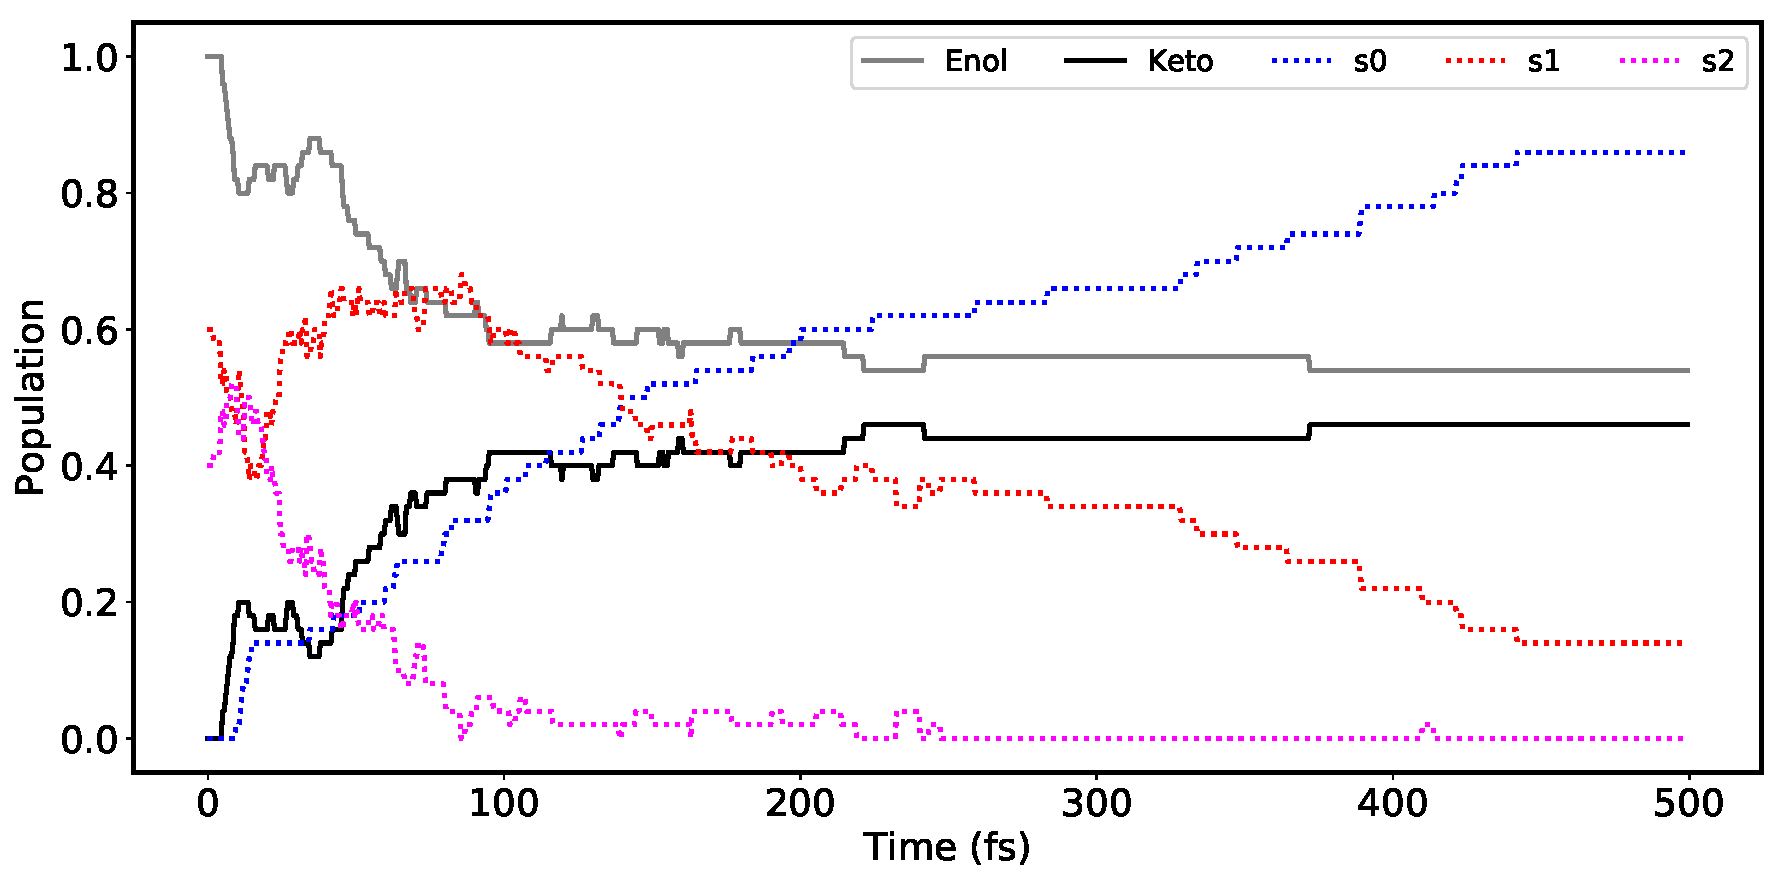
\includegraphics[width=0.9\linewidth]{3nonradiativedecay/HC_1_populations.pdf}
  \caption[Populations of \textbf{HC1} in nonadiabatic dynamics simulations]{The population of the \szero{}, \sone{}, and \stwo{} states for compound \textbf{1} from \ac{TSH} simulations. The population of enol and keto states are also shown.}
  \label{figure: HC_1_Populations}
\end{figure}

\begin{figure}[H]
\centering
  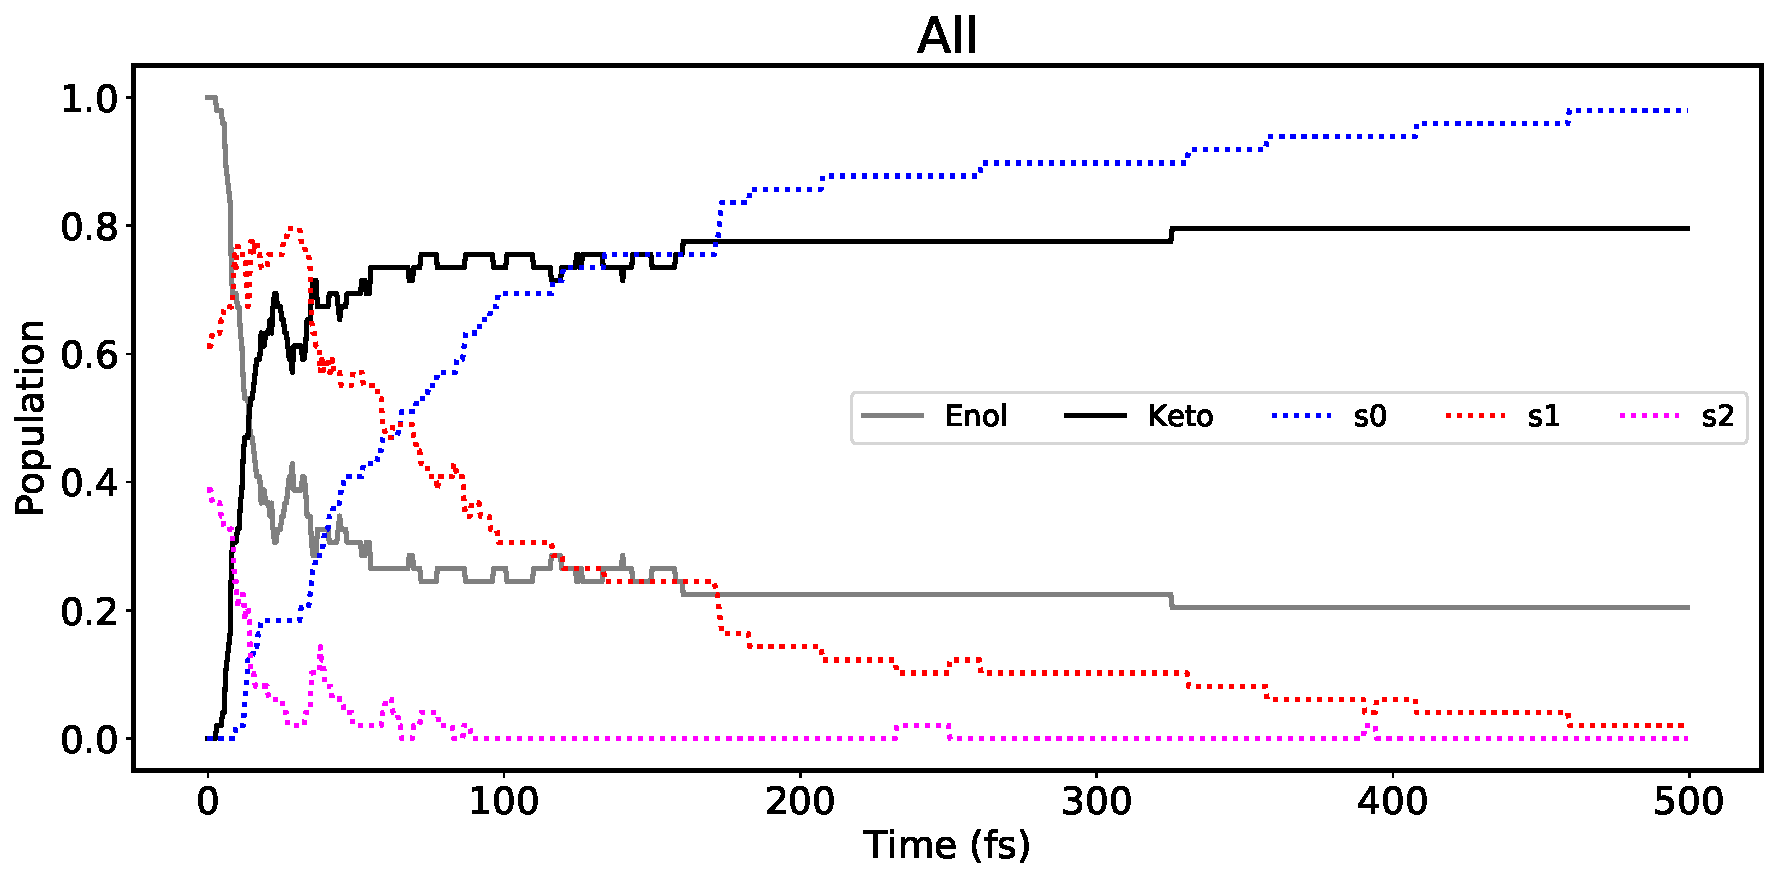
\includegraphics[width=0.9\linewidth]{3nonradiativedecay/HC_5_populations.pdf}
  \caption[Populations of \textbf{HC5} in nonadiabatic dynamics simulations]{The population of the \szero{}, \sone{}, and \stwo{} states for compound \textbf{1} from \ac{TSH} simulations. The population of enol and keto states are also shown.}
  \label{figure: HC_5_Populations}
\end{figure}

The decay rate of the \Estar{} state was estimated by assuming first-order kinetics, where for each time step the enol population was calculated based on the O-H bond length for each trajectory. The reaction scheme proposed is:
\begin{align*}
\centering
\ce{&E^{*} ->[$K_{1}$] K^{*}\\&E^{*} ->[$K_{2}$] E}
\end{align*}
with a combined rate constant of $K=K_{1}+K_{2}$, incorporating both ESIPT and internal conversion decay mechanisms. The fit of $K$, the \Estar{} decay rate, for \textbf{1} and \textbf{5} is shown in Figure \ref{figure: HC_Dynamics_Enolfit}. In \textbf{1}, $K=0.0154$ fs\textsuperscript{-1}, giving a lifetime of just 65 fs. For compound \textbf{5} the lifetime is even shorter at just 18 fs. Whilst these times are certainly underestimated, they show the instability of the enol state for \textbf{5} compared to \textbf{1}. While the goodness of fit is reasonable, at 0.74 and 0.81 respectively for \textbf{1} and \textbf{2} (Figure \ref{figure: HC_Dynamics_Enolfit}), the largest error comes from combining the nonradiative decay rate and the ESIPT rate into one decay constant. Furthermore, it can be seen that there are many unphysical step-like features in the populations. Both of these factors are a result of the relatively small number of trajectories run. More accurate lifetimes could thus be attained by running more trajectories and with a higher level of theory to better sample the phase space and allow the separation and estimation of $K_{1}$ and $K_{2}$. However the computational cost associated with this is prohibitive, and for a qualitative description the current method shows the relative differences of the compounds. Besides the elevated computational costs, there are known problems with the stability of CC2 for dynamics.\cite{Plasser2014}

\begin{figure}[t]
\centering
  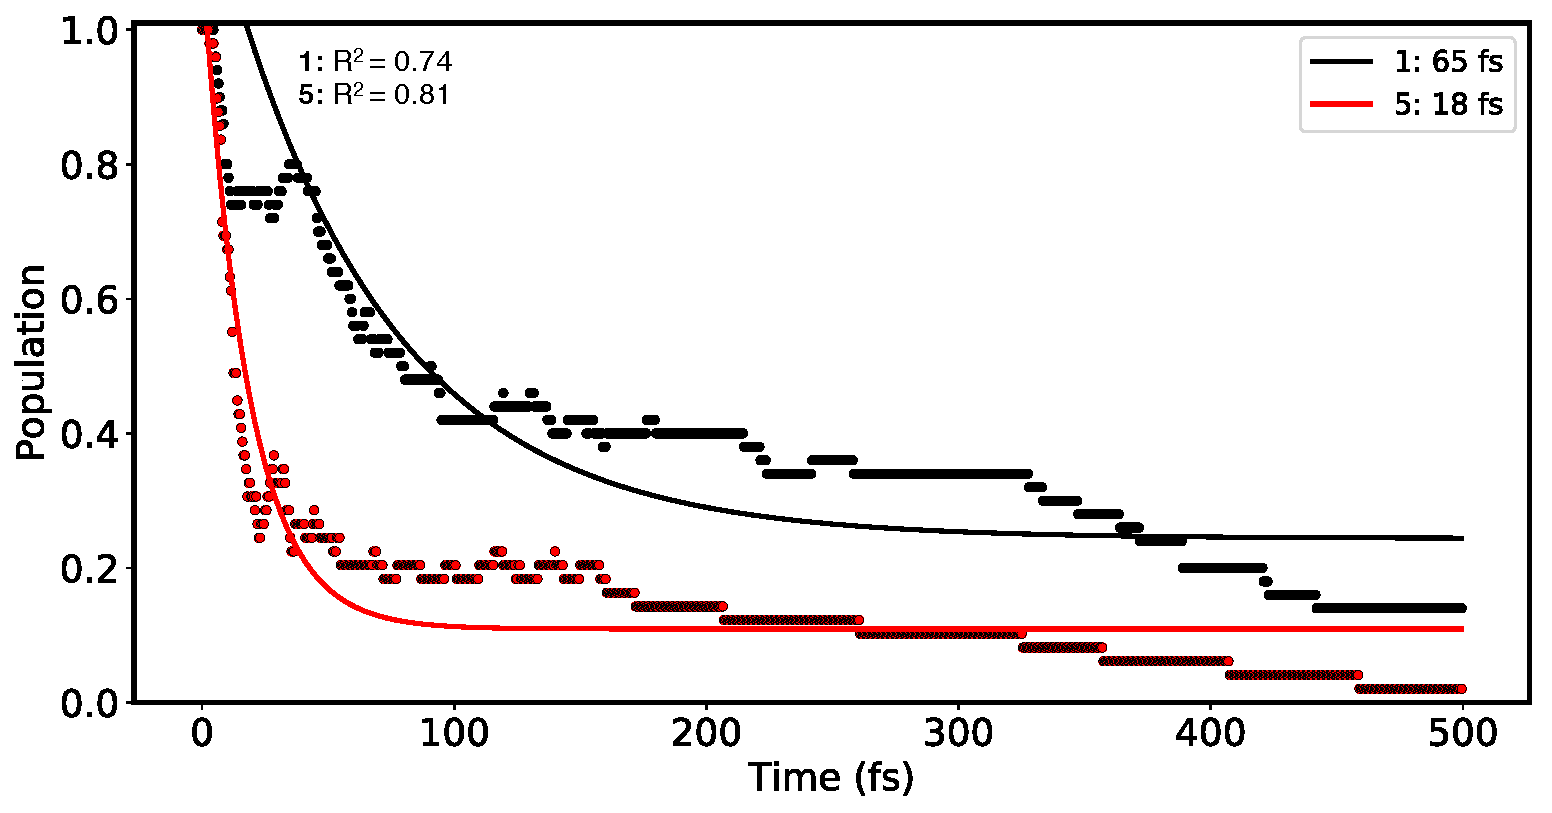
\includegraphics[width=0.9\linewidth]{3nonradiativedecay/HC_dynamics_enolfit.pdf}
  \caption[Estimation of enol decay rate]{Estimation of the enol lifetime for \textbf{1} and \textbf{5} using first-order exponential decay.}
  \label{figure: HC_Dynamics_Enolfit}
\end{figure}

The lifetimes of \stwo{} and \sone{} were also estimated using a consecutive reaction scheme,
\begin{align*}
\centering
\ce{&S_{2} ->[$K_{A}$]S_{1} ->[$K_{B}$] S_{0}}
\end{align*}
where the lifetime fits are shown in Figures \ref{figure: HC_1_states_dynamics_fit} and \ref{figure: HC_5_states_dynamics_fit}. In compound \textbf{1}, there is slight population transfer from \sone{} to \stwo{} that is not included in the model and thus decreases the quality of the \sone{} fit. Nevertheless, in both compounds there is fast population transfer from \stwo{} to \sone{}, followed by a longer-lived \sone{} state. In \textbf{1}, the lifetime of 215 fs ($K_{B}=0.0047$ fs\textsuperscript{-1}) dwarfs that of compound \textbf{5} ($K_{B}=0.0103$ fs\textsuperscript{-1}), again underscoring the power of the methoxy group to destabilise the excited state. The greater stability of \sone{} for compound \textbf{1} can be attributed to the stability of the \Estar{} channel, where seven trajectories remain beyond the 500 fs simulation time. For compound \textbf{5}, just one trajectory remained active at 500 fs, in the enol state.

\begin{figure}[H]
\centering
  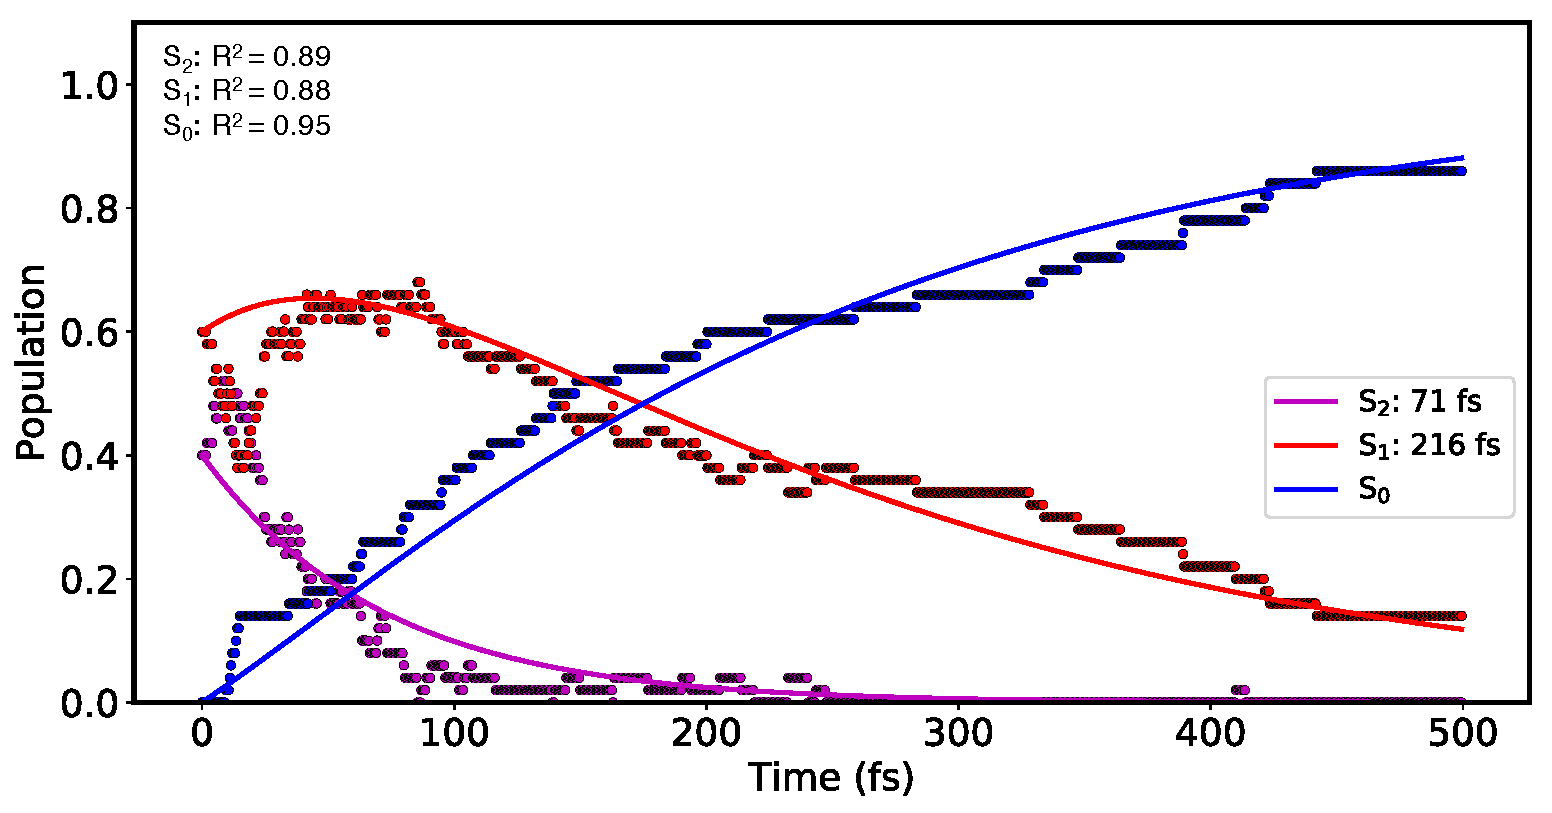
\includegraphics[width=0.9\linewidth]{3nonradiativedecay/HC_1_states_dynamics_fit.pdf}
  \caption[Model of the state decay rates for \textbf{HC1}]{Fit of the rate constants for excited state decay of \stwo{}, \sone{}, and \szero{} for compound \textbf{1}.}
  \label{figure: HC_1_states_dynamics_fit}
\end{figure}

\begin{figure}[H]
\centering
  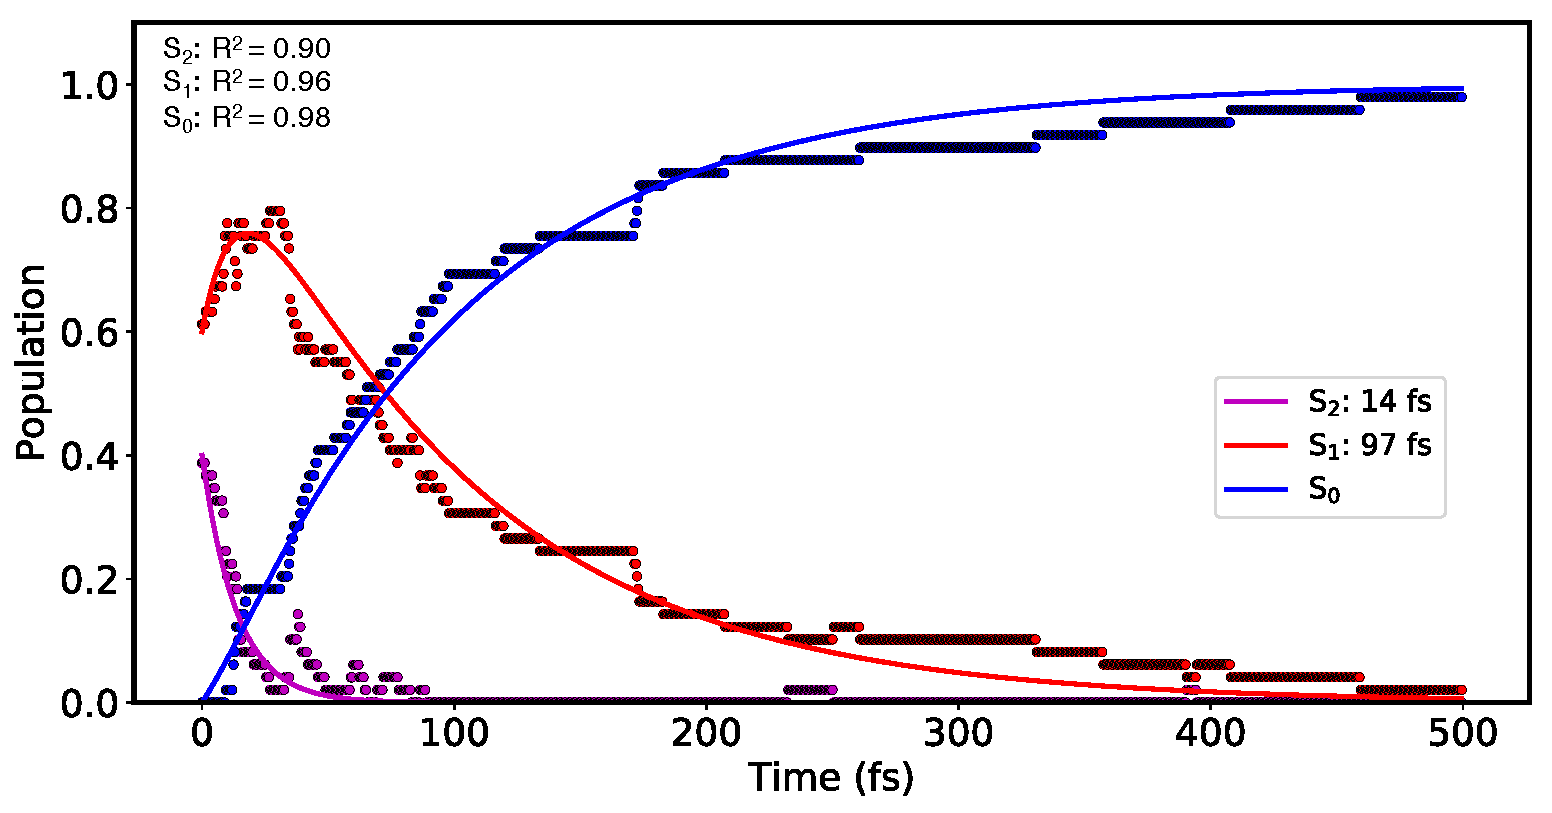
\includegraphics[width=0.9\linewidth]{3nonradiativedecay/HC_5_states_dynamics_fit.pdf}
  \caption[Model of the state decay rates for \textbf{HC5}]{Fit of the rate constants for excited state decay of \stwo{}, \sone{}, and \szero{} for compound \textbf{5}.}
  \label{figure: HC_5_states_dynamics_fit}
\end{figure}


For \textbf{1} and \textbf{5}, the average time for the first proton transfer is 59 fs and 10 fs respectively, with all trajectories exhibiting ESIPT finding the ground state before the maximum simulation time (500 fs). We identify three steps in the ESIPT mechanism:
\begin{enumerate}
    \item Relaxation in the excited state (\Estar{} form)
    \item Proton transfer (ESIPT) 
    \item Relaxation in \Kstar{} followed by internal conversion
\end{enumerate}

These three steps are illustrated for a typical trajectory in panel a) of Figure \ref{figure: HC_1_Trajectories}. During step 1, the angle decreases to $\theta_{tor}$=11\textdegree{} to facilitate the proton transfer in step 2. In some trajectories, the proton oscillates somewhat before transferring. ESIPT in step 2 occurrs at 45 fs. In step 3, the molecule relaxes in the keto form \textit{via} dihedral rotation after which dihedral rotation of 37\textdegree{} results in state convergence after 139 fs, which is underestimated considering the limitations of the ADC(2) method. The region with \sone/\szero{} gap of 0.1 eV is accessed in an average time of 76 fs post-ESPIT for \textbf{1} and 47 fs for \textbf{5}. Considering the features of the PES at ADC(2)/def2-SV(P) level of theory, these times are underestimated with respect to real internal conversion times, but they provide a relative indication of how fast the molecules reach the crossing seam region and the effect of the substituent.
\begin{figure}[t]
\centering
  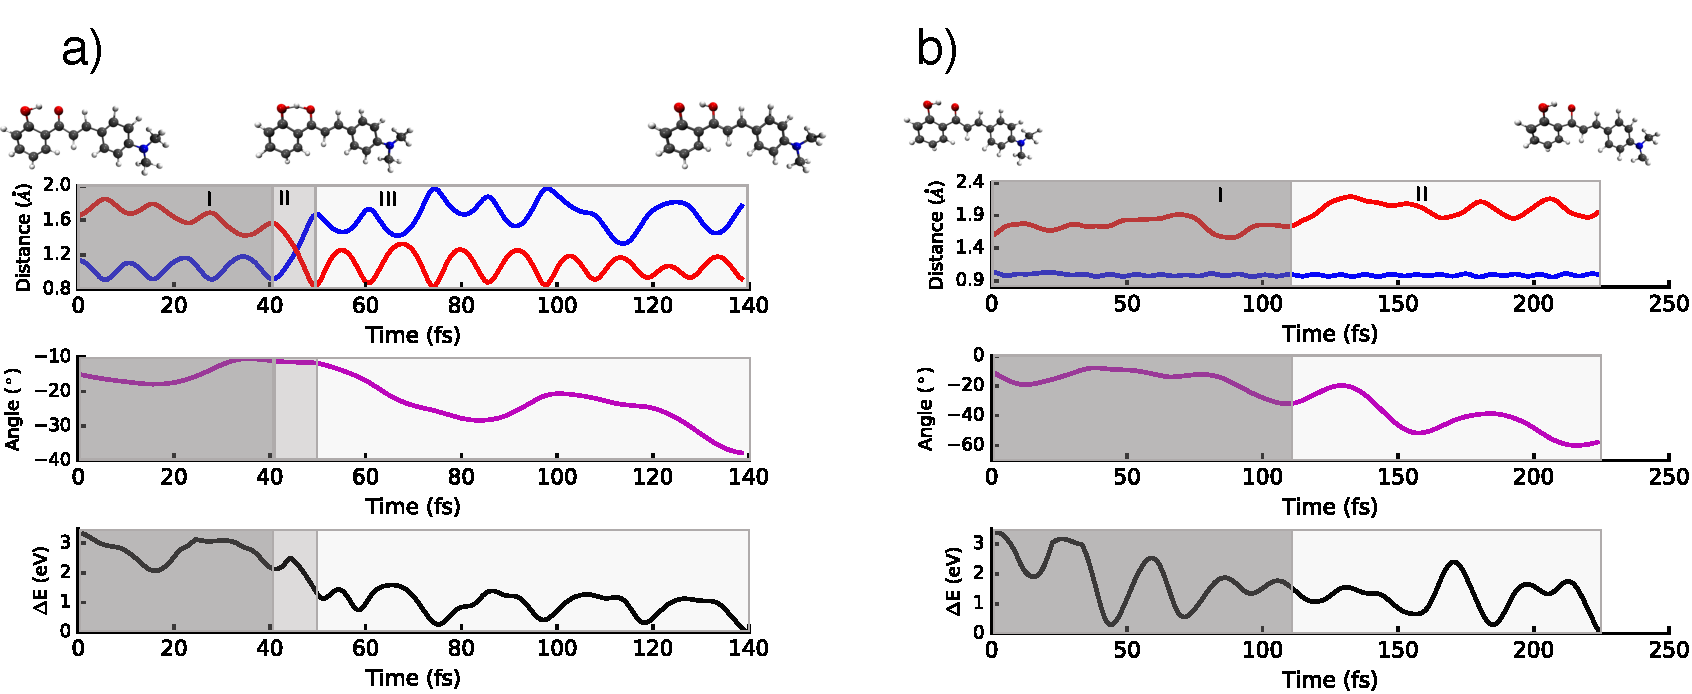
\includegraphics[width=0.9\linewidth]{3nonradiativedecay/HC_1_Trajectories.pdf}
  \caption[Typical trajectories for \textbf{HC1}]{Two exemplar trajectories of compound \textbf{1}. Panel a), left, shows a trajectory undergoing ESIPT, with the associated O-H distances, dihedral angle, and energy gap between \sone{} and \szero{}. The same parameters are shown in panel b) for a trajectory which relaxes in the \Estar{} channel.}
  \label{figure: HC_1_Trajectories}
\end{figure}

Alternatively to ESIPT, the molecule can remain in the \Estar{} state. The mechanism of intramolecular rotation in \Estar{} compromises two steps: 
\begin{enumerate}
    \item Relaxation in the \Estar{} minimum, which is close to the Franck-Condon geometry.
    \item Further relaxation leading to the internal conversion
\end{enumerate}
Both processes involve the rotation around the angle $\theta_{tor}$. 20\% of the trajectories deactivated through this channel did not reach the crossing region within the simulation time. In the case of \textbf{5}, where there is not a \Estar{} minimum close to the Franck-Condon geometry, the molecule relaxes directly to the crossing seam region. On average, the crossing region is reached within  228 fs for \textbf{1} and 241 fs for \textbf{5}. 

In panel b) of Figure \ref{figure: HC_1_Trajectories}, a typical trajectory undergoing \Estar{} relaxation is shown. At 0 fs,  $\theta_{tor}$=-10.5\textdegree{}, and for the first 110 fs of the simulation (step 1), the angle oscillates about the equilibrium value (-11.0\textdegree{} at ADC(2)/def2-SV(P) level of theory). Then, the rotation deviates the phenoxy group from the plane prohibiting ESIPT and the molecule reaches the CI region at 225 fs, with an $\theta_{tor}$=-57.6\textdegree{}. The dynamics support the assertions from the \acp{PES} that proton transfer from the twisted \Estar{} form, with a barrier of 1.2 eV, is improbable. Relaxation in \Estar{} therefore competes with ESIPT in compound \textbf{1} due to the close proximity of a local minimum close to the Franck-Condon geometry. Proton transfer followed by internal conversion is the faster process, with an average time duration of 123 fs, compared to 228 fs for rotation in \Estar{}.

The nonadiabtic dynamic simulations do not allow the prediction of post-internal conversion behaviour, but the analysis of the PES can help understand the following steps in the mechanisms. Post-ESIPT, two relaxation pathways are possible once the MECI is populated. The first completes the four-level photocycle and returns the system to the ground state cis-enol form \textit{via} \ac{GSIPT}. The second continues the rotation about $\theta_{tor}$ to produce the trans-keto form of \textbf{HC}.  Optimisation at the MP2/def2-TZVP level show this structure is more than 1 eV less stable than the ground state, suggesting that \ac{GSIPT} will be preferential. This is shown schematically in Figure \ref{figure: HC_1_Energylevels_ADC2}. The nonadiabatic dynamics simulations clearly illustrate the effect of a strong electron donor in the \textit{para} position on the ESIPT process in \ac{HC}s. The population of the ESIPT channel and rate of proton transfer is greatly increased as is subsequent convergence of the ground and first excited state. 

\begin{figure}
\centering
  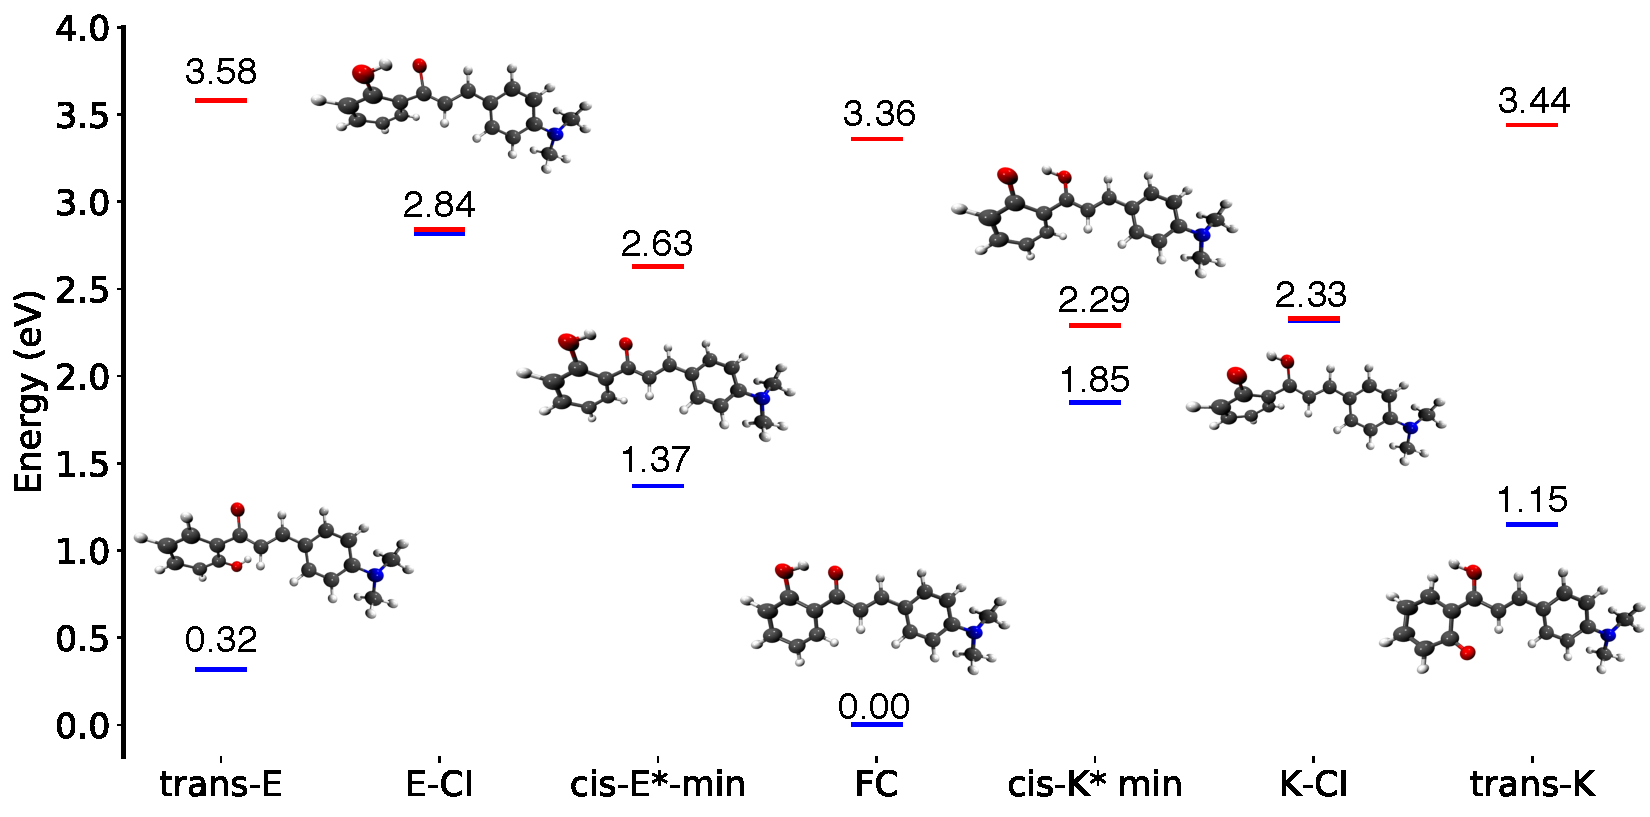
\includegraphics[width=0.9\linewidth]{3nonradiativedecay/HC_1_energylevels_ADC2.pdf}
  \caption[Energies of important optimised states for \textbf{1}]{Energies of important optimised energies on the \ac{PES} of \textbf{1}. Ground states optimised at MP2/def2-TZVP, whilst excited state minima optimised at ADC(2)/def2-TZVP level of theory.}
  \label{figure: HC_1_Energylevels_ADC2}
\end{figure}

\section{Conclusions}\label{section: NRdecay_Conclusions}
In this chapter computational methods have been applied to investigate the photochemistry of five derivatives of \ac{HC}, an ESIPT-active compound with potential application in organic lasers and optoelectronics. Experimental data show that \ac{HC}s are non-emitting in solution and only fluoresce through \ac{AIE}.\cite{Cheng2015} The calculations provide theoretical description of the ESIPT process and subsequent relaxation mechanisms of \ac{HC}s in gas phase, which represents the first step for the understanding of the photochemistry of these systems. 

Through calculation of vertical excitation energies and corresponding absorption spectra, we find that electron donating groups have but a small influence of the absorption characteristics of \ac{HC}. It takes a strong electron donor in the \textit{para} position to alter the vertical excitation energy, on account of the increased conjugated electron density. On the other hand, relaxation back to the ground state is far more sensitive to the electron donating power of the substituent and its positioning on the phenol moiety. Dual-emission is inhibited with an EDG in \textit{para} for \ac{HC}s. This is quite unexpected, with a comprehensive study on the effects of substituents in common ESIPT-compounds finding that electron donating groups in any position favour the \Estar{} form, showing the complex nature of ESIPT chromophores.\cite{Azarias2016}

The ground state is accessible \textit{via} non-radiative channels from both \Estar{} and \Kstar{} states. \sone/\szero{} MECI structures were found for all compounds, associated with an extended crossing seam. Both mechanisms involve the activation of an intermolecular rotation mode about the $\theta_{tor}$ angle. The competition between both mechanisms depends strongly on the position and nature of the substituent of the substituent. Proton transfer is more favourable with electron donating groups in \textit{para}, correlating with donating power and increased electron density loss at the phenol oxygen. Nonadiabatic surface-hopping dynamic simulations provide a full picture of relaxation energetics and timescales. 

ESPIT is strongly favoured for \textbf{4}-\textbf{5}, where there are not stable \Estar{} minima. For compound \textbf{5}, the reaction coordinate is completely downhill correlating with intramolecular rotation. The dynamic simulations show a bias towards the \Kstar{} relaxation mechanism. Experimentally, \textbf{4} and \textbf{5} do not fluoresce either in solution or solid state. Cheng \textit{et al.} suggested that for the solid material, this behaviour is related to the crystal packaging.\cite{Cheng2015} Our calculations show that the character of the substituent and the electronic effects in the monomers might also play a role in the mechanism. In the next chapter the knowledge of the electronic properties of \textbf{1} and \textbf{5} shall be used to probe the excited state decay process in the molecular crystal. The question remains of why \textbf{5} is still nonemissive in the solid state whilst \textbf{1} undergoes a stitch-on of fluorescence. To probe this, we shall examine the intermolecular interactions in the molecular crystal and their importance in relation to the electronic properties of the chromophore. 



